\documentclass{beamer}
\usepackage[utf8]{inputenc}

\usetheme{Madrid}
\usecolortheme{default}
\usepackage{amsmath,amssymb,amsfonts,amsthm}
\usepackage{txfonts}
\usepackage{tkz-euclide}
\usepackage{listings}
\usepackage{adjustbox}
\usepackage{array}
\usepackage{tabularx}
\usepackage{gvv}
\usepackage{lmodern}
\usepackage{circuitikz}
\usepackage{tikz}
\usepackage{graphicx}
\usepackage{mathtools}

\setbeamertemplate{page number in head/foot}[totalframenumber]

\usepackage{tcolorbox}
\tcbuselibrary{minted,breakable,xparse,skins}



\definecolor{bg}{gray}{0.95}
\DeclareTCBListing{mintedbox}{O{}m!O{}}{%
  breakable=true,
  listing engine=minted,
  listing only,
  minted language=#2,
  minted style=default,
  minted options={%
    linenos,
    gobble=0,
    breaklines=true,
    breakafter=,,
    fontsize=\small,
    numbersep=8pt,
    #1},
  boxsep=0pt,
  left skip=0pt,
  right skip=0pt,
  left=25pt,
  right=0pt,
  top=3pt,
  bottom=3pt,
  arc=5pt,
  leftrule=0pt,
  rightrule=0pt,
  bottomrule=2pt,
  toprule=2pt,
  colback=bg,
  colframe=orange!70,
  enhanced,
  overlay={%
    \begin{tcbclipinterior}
    \fill[orange!20!white] (frame.south west) rectangle ([xshift=20pt]frame.north west);
    \end{tcbclipinterior}},
  #3,
}
\lstset{
    language=C,
    basicstyle=\ttfamily\small,
    keywordstyle=\color{blue},
    stringstyle=\color{orange},
    commentstyle=\color{green!60!black},
    numbers=left,
    numberstyle=\tiny\color{gray},
    breaklines=true,
    showstringspaces=false,
}
\title{10.7.94}
\date{1st October, 2025}
\author{Puni Aditya - EE25BTECH11046}

\begin{document}

\frame{\titlepage}
\begin{frame}{Question}
A circle touches the X axis and also touches the circle with centre at \brak{0, 3} and radius 2. The locus of the centre of the circle is
\begin{enumerate}
    \item an ellipse
    \item a circle
    \item a hyperbola
    \item a parabola
\end{enumerate}
\end{frame}

\begin{frame}{Theoretical Solution}
Let the center of the moving circle be $\vec{c}$ and its radius be $r$.
The circle touches the X-axis, so its radius is the y-coordinate of its center.
\begin{align}
    r = \vec{e_2}^\top\vec{c} \text{ } \brak{\text{assuming } \vec{e_2}^\top\vec{c}>0}
\end{align}
The fixed circle has center $\vec{c}_f$ and radius $r_f$. The distance between the centers of two externally touching circles is the sum of their radii.
\begin{align}
    \norm{\vec{c}-\vec{c}_f} &= r + r_f \\
    \norm{\vec{c}-\vec{c}_f} &= \vec{e_2}^\top\vec{c} + r_f
\end{align}
\end{frame}

\begin{frame}{Theoretical Solution}
Squaring both sides,
\begin{align}
    \brak{\vec{c}-\vec{c}_f}^\top\brak{\vec{c}-\vec{c}_f} &= \brak{\vec{e_2}^\top\vec{c} + r_f}^2 \\
    \vec{c}^\top\vec{c} - 2\vec{c}_f^\top\vec{c} + \vec{c}_f^\top\vec{c}_f &= \brak{\vec{e_2}^\top\vec{c}}^2 + 2r_f\brak{\vec{e_2}^\top\vec{c}} + r_f^2
\end{align}
Rearranging to the matrix quadratic form $\vec{c}^\top\vec{V}\vec{c} + 2\vec{u}^\top\vec{c} + f = 0$:
\begin{align}
    \vec{c}^\top\brak{\vec{I}-\vec{e_2}\vec{e_2}^\top}\vec{c} + 2\brak{-\vec{c}_f - r_f\vec{e_2}}^\top\vec{c} + \brak{\vec{c}_f^\top\vec{c}_f-r_f^2} = 0
\end{align}
\end{frame}

\begin{frame}{Theoretical Solution}
The given values are $\vec{c}_f = 3\vec{e_2}$ and $r_f=2$.
\begin{align}
    \vec{V} &= \vec{I} - \vec{e_2}\vec{e_2}^\top = \myvec{1 & 0 \\ 0 & 1} - \myvec{0 & 0 \\ 0 & 1} = \myvec{1 & 0 \\ 0 & 0} \\
    \vec{u} &= -\vec{c}_f - r_f\vec{e_2} = -3\vec{e_2} - 2\vec{e_2} = -5\vec{e_2} = \myvec{0 \\ -5} \\
    f &= \vec{c}_f^\top\vec{c}_f - r_f^2 = \brak{3\vec{e_2}}^\top\brak{3\vec{e_2}} - 2^2 = 9 - 4 = 5
\end{align}
The locus in the standard form of the conic is
\begin{align}
    \vec{c}^\top\myvec{1 & 0 \\ 0 & 0}\vec{c} + 2\myvec{0 & -5}\vec{c} + 5 = 0
\end{align}
\end{frame}

\begin{frame}{Theoretical Solution}
The type of conic section is determined by the eigenvalues of $\vec{V}$. For a diagonal matrix, the eigenvalues are the diagonal entries.
\begin{align}
    \lambda_1 = 1, \text{ } \lambda_2 = 0
\end{align}
\begin{align}
    \mydet{\vec{V}} = \lambda_1\lambda_2 = 1 \cdot 0 = 0
\end{align}
Since one of the eigenvalues is zero, the locus is a parabola. \\
The correct option is \textbf{4) a parabola}.
\end{frame}

\begin{frame}{Plot}
\begin{figure}
    \centering
    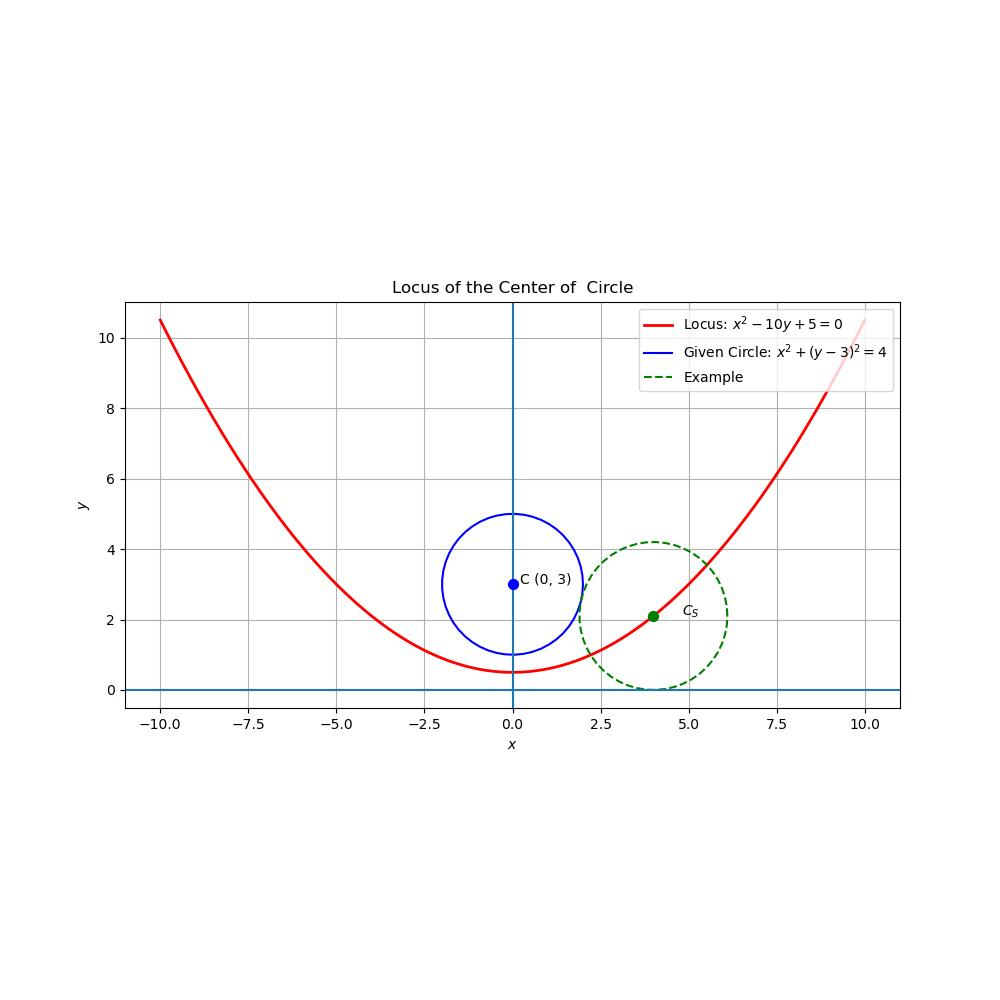
\includegraphics[width=0.5\columnwidth]{../figs/plot_c.jpg}
    \caption{Plot}
    \label{fig:fig}
\end{figure}
\end{frame}

\end{document}
